% !TeX spellcheck = en_US
\documentclass[a4paper]{report}
\usepackage[T1]{fontenc}
\usepackage[utf8]{inputenc}
\usepackage[english]{babel}
\usepackage{geometry}
\usepackage{graphicx}
\usepackage{subfig}
\geometry{a4paper,top=2.5cm,bottom=2.5cm,left=3cm,right=3cm,%
	heightrounded,bindingoffset=5mm}
\begin{document}

\title{\Huge{JustRecipe}}
\author{\Large{Francesco Campilongo - Daniele Cioffo - Francesco Iemma}}
\date{Academic Year 2020/21}
\maketitle
\tableofcontents

\chapter*{Introduction}

\chapter{Dataset}
In this first chapter of this document we will talk about searching for the initial dataset.

\noindent As specified in the project documentation, the dataset had to be at least 50MB large, and this quantity could not be generated directly within the application. So we did an initial search, finding two datasets, which were generated by their authors by performing the scraping on the sites \emph{www.FoodNetwork.com} and \emph{www.Epicurios.com}. The second dataset was more complete (more nutritional values), so it was used as the main dataset. The other dataset was used to complement the other, reaching a total of  67.8 MB, with 45349 recipes.

\noindent To correctly extract the data present in the two datasets we wrote a program in Java, called \emph{RecipeReade}r, thanks to which we adapted the two different formats and removed the duplicates (recipes with the same title that were present in both datasets).
To implement this program we used the GSon library and the Jackson library.

\noindent The variety property is ensured by using two different sources. The velocity / variability properties are ensured because comments and recipes are eliminated and added inside the application, indeed this data may lose importance after a certain time interval since new data quickly arrives.

\chapter{Design}
\section{Introduction To The Application}
The topic of cuisine is extensively widespread in our society. In fact we can think at the success achieved by tv shows related to cooking in the last years and also at the fact that a lot of chefs are becoming superstars.
Then there is another important factor: the coronavirus outbreak.

\noindent With the coronavirus outbreak a lot of people became cuisine lovers, in fact at the first moments of the pandemia several ingredients as flour and yeast were very hard to find, because people were confined in their home and so they had more free time.

\noindent But this topic is not a recente one. The first recipe book dates back to eigth century B.C. and it is the so-called \emph{Eraclio} (by the name of the city in which he was found). Then also an important latin writer, Apicio, wrote one of the most important recipe books of the roman era: \emph{De Re Coquinaria} which dates back to the first century B.C..
 
\noindent So the topic of cuisine is inherent to human nature, because the necessity of eating is a basic need.
Furthermore, everyone has experimented the infamous question: “What will I eat this evening?”. JustRecipe has the aim of answer to this question, it has the aim of helping university student or workers to retrieve and to do fast and simple recipes.

\noindent So this application is basically a recipe book but it is also more than this.

\noindent JustRecipe is also a social network which allow people to enjoy, to ex-change ideas about cooking, to feel less lonely in this hard period.

\section{Requirements}
\subsection{Main Actors}
The main actors of the application are four:
\begin{itemize}
	\item Unregistered User
	
	\noindent He is the user which open the application for the first time, in order to access he must sign-up.
	
	\item User
	
	\noindent He is the normal user (the registered one).
	
	\item Moderator
	
	\noindent He is in charge of controlling the comments and eventually delete the ones which contain abuses.
	
	\item Administrator
	
	\noindent He is the most powerful actor, he can delete users and recipes and he is also in charge of elect moderators
\end{itemize}

\noindent Each actor can do all the features of the previous ones in the list.

\subsection{Functional Requirements}
\subsubsection{Features offered to the Unregistered User}
\begin{itemize}
	\item  Registration
	
	\noindent In order to access the application an user must sign-up. Otherwise he is not allowed to access and to use all the functionalities.
\end{itemize}
\subsubsection{Features offered to the Registered User}
\begin{itemize}
	\item Login/Logout
	
	\noindent The only way to access the application, as we said previously, is to sign-up and the login. At the end the user can logout and close the session.
	
	\item Search a recipe
	
	\noindent It's possible to search a recipe searching for the title and for categories.
	
	\item Browse suggested recipes
	
	\noindent The suggestions will be offered in a proper section, they are done considering the relationship between the user logged, the users followed by the user logged and so on so forth.
	
	\item Browse recipes of following users
	
	\noindent In a proper section (i.e. the Homepage) the user can browse the recipes of the following user. Indeed he can see only a snapsht of the recipes, if he want a more in-depth view he can click on it and se the recipe page in which he is able to see all the recipe details. 
	
	\item Add a recipe
	\item Edit own recipes
	\item Comment recipes
	\item Follow another user
	\item Like a recipe
\end{itemize}

\subsubsection{Features offered to the Moderator}
\begin{itemize}
	\item Delete comments
	
	\noindent The moderator is in charge of delete comments which contain racist abuse, crude terms and so on so forth.
\end{itemize}

\subsubsection{Features offered to the Administrator}
\begin{itemize}
	\item Delete users
	\item Delete recipes
	\item Elect moderators
\end{itemize}
\subsection{Non-Functional Requirements}

\subsection{Actors and Use Cases}
The use case diagram of the application is described in the figure 2.1 
\begin{figure}[htpb]
	\centering
	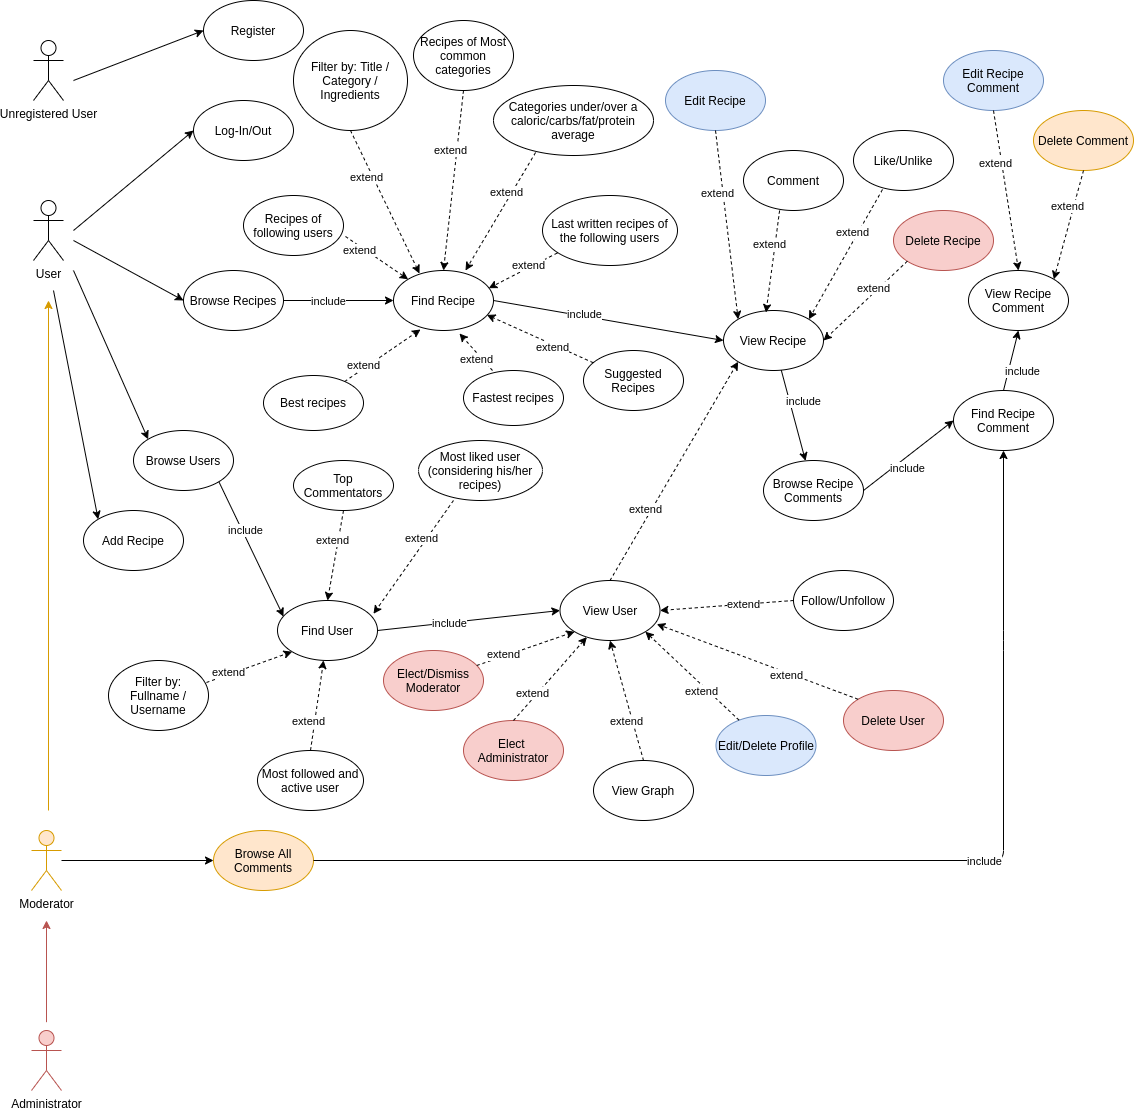
\includegraphics[scale=0.5]{img/UseCaseDiagram.png}
	\caption{Use Case Diagram}
\end{figure}
\section{UML Class Diagram}
\section{Data Model}
\subsection{DocumentDB}
\subsection{GraphDB}
\section{Distributed Database Design}
\subsection{Replicas}
\subsection{Sharding}
\section{Software Architecture}


\chapter{Implementation and Test}
\section{Main Modules}
\section{Main Packages and Classes}
\section{Most Relevant Queries}
\subsection{MongoDB}
\subsection{Neo4J}
\section{Unit Test}
\section{Tests and Statistical Analysis}

\chapter{User Manual}
\end{document}
